\documentclass{BeamerTemplate}
\title{Module 2 - Variables aléatoires à une dimension}
\subtitle{STT-1000 Probabilités et statistique}
\date{\today}

% Lien discret vers la page de réponses, ajouté au pied de page à côté du numéro
% (ne prend aucune place sur la diapo). Usage, n'importe où dans la diapo : \lienreponse{rep-ex1}
\newcommand{\cibleReponse}{}
\newcommand{\lienreponse}[1]{\gdef\cibleReponse{#1}}
\addtobeamertemplate{footline}{}{%
  \ifx\cibleReponse\empty\else
    \begin{tikzpicture}[remember picture,overlay]
      \node[anchor=south east, inner sep=0pt] at ([xshift=-1.5cm,yshift=0.2cm]current page.south east)
        {\hyperlink{\cibleReponse}{\scriptsize\color{gray}Réponse~$\rightarrow$}};
    \end{tikzpicture}%
    \global\let\cibleReponse\empty
  \fi}
% Lien de retour vers l'exemple, dans les pages de réponses
\newcommand{\retour}[2]{\hyperlink{#1}{\textbf{#2}~{\color{gray}$\hookleftarrow$}}}

% Graphiques de la loi exponentielle (exemples 3 et 6) : λ = 1, 1/3 et 1/10
\pgfplotsset{
  expo/.style={
    width=6.6cm, height=4.4cm, axis lines=left, xmin=-2, xmax=19,
    xtick={0,5,10,15}, tick label style={font=\tiny}, label style={font=\scriptsize},
    xlabel={$x$ = temps de réponse (ms)}, samples=120,
    legend style={font=\tiny, draw=none, fill=none}, legend cell align=left,
  },
}

% Densité illustrative de la diapo « Probabilité = aire sous la densité »
\pgfmathdeclarefunction{dens}{1}{\pgfmathparse{0.2756*sqrt(#1-1)*(9-#1)}}

\begin{document}
\begin{frame}[t]
  \titlepage
\end{frame}

\section{Introduction}
\begin{frame}[t]{Exemple 1}
Le résultat d'une expérience aléatoire est souvent un nombre réel. Sinon, on peut associer un nombre réel à chacun de ses résultats possibles.

\medskip
{\ }

\uncover<2->{
 $\mathcal{E}$ : on lance une pièce de monnaie 2 fois.

 $\mathcal{U}=\{FF,FP,PF,PP\}$.

 \medskip
 Par exemple, on peut associer à chaque résultat le nombre de fois où pile apparaît. Notons $X$ cette variable :

 \begin{tabular}{ll}
 $X=0$ & si le résultat est $FF$,\\
 $X=1$ & si le résultat est $FP$ ou $PF$,\\
 $X=2$ & si le résultat est $PP$.
 \end{tabular}
}
\end{frame}

\begin{frame}{Variable aléatoire}

Soit $\mathcal{E}$ une expérience aléatoire d'espace échantillonnal $\mathcal{U}$.

 \begin{Boite}{Variable aléatoire}
On appelle \alerter{variable aléatoire} (v.a.) toute fonction $X$ qui associe un nombre réel $X(e)$ à chaque élément $e\in \mathcal{U}$.

\medskip

L'ensemble des valeurs que peut prendre $X$ est noté $\mathbb{R}_X$ et s'appelle l'\alerter{image de $X$}.
 \end{Boite}
On désigne habituellement une v.a. par une lettre majuscule et ses valeurs par une lettre minuscule. Par exemple, $P(X=x)$ est la probabilité que la variable aléatoire $X$ prenne la valeur $x$.

\end{frame}

\begin{frame}[t,label=ex2]{Exemple 2}

$\mathcal{E}$ : on lance un dé équilibré et on observe la face du dessus. \\
$\mathcal{U}=\{1,2,3,4,5,6\}$.\\
On peut définir une infinité de variables aléatoires sur cette expérience.
En voici deux.

 \begin{itemize}
  \item<2-> $X$ est le résultat observé :\\
    $X(e)=e,~\forall e\in \mathcal{U}$\\
    $\mathbb{R}_X=\{1,2,3,4,5,6\}$
  \item<3-> Je gagne 1~\$ si j'obtiens 4, 5 ou 6.\\
    Je perds 1~\$ si j'obtiens 1, 2 ou 3.\\
    $Y$ est mon gain :\\
      $Y(e)=\left\{
  \begin{array}{rl}
  -1 &\text{si}\;e\in\{1,2,3\}\\
  1&\text{si}\;e\in\{4,5,6\}
  \end{array}
  \right.$\\
  $\mathbb{R}_Y=\{-1,1\}$.
 \end{itemize}
\end{frame}

\begin{frame}[t,label=ex2tab]{Exemple 2 (suite)}

\begin{columns}[T]
\begin{column}{0.36\textwidth}
{\large
 \begin{tabular}{c|c|c}\hline
 $e$ & $X(e)$ & $Y(e)$ \\ \hline
  1 & & \\
  2 & & \\
  3 & & \\
  4 & & \\
  5 & & \\
  6 & & \\ \hline
 \end{tabular}
}
\end{column}
\begin{column}{0.6\textwidth}
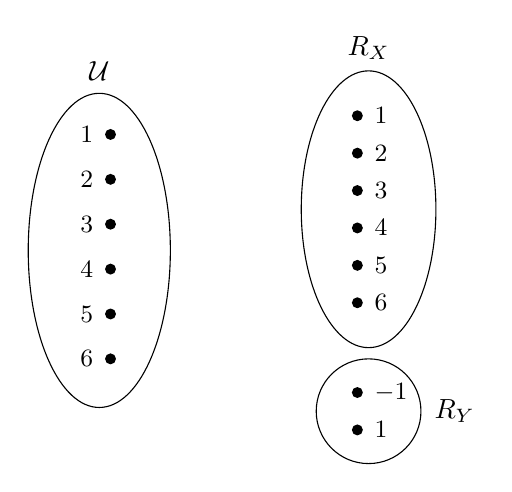
\begin{tikzpicture}[scale=0.95, pt/.style={circle, fill, inner sep=1.4pt}]
  % Espace échantillonnal
  \draw (0,0.2) ellipse (0.95 and 2.1);
  \node at (0,2.6) {$\mathcal{U}$};
  \foreach \i in {1,...,6} {
    \node[pt] at (0.15,2.05-0.6*\i+0.3) {};
    \node[left] at (0.05,2.05-0.6*\i+0.3) {\small \i};
  }
  % Image de X
  \draw (3.6,0.75) ellipse (0.9 and 1.85);
  \node at (3.6,2.9) {$\mathbb{R}_X$};
  \foreach \i in {1,...,6} {
    \node[pt] at (3.45,2.5-0.5*\i) {};
    \node[right] at (3.55,2.5-0.5*\i) {\small \i};
  }
  % Image de Y
  \draw (3.6,-1.95) circle (0.7);
  \node at (4.75,-1.95) {$\mathbb{R}_Y$};
  \node[pt] at (3.45,-1.7) {}; \node[right] at (3.55,-1.7) {\small $-1$};
  \node[pt] at (3.45,-2.2) {}; \node[right] at (3.55,-2.2) {\small $1$};
\end{tikzpicture}
\end{column}
\end{columns}
\lienreponse{rep-ex1}
\end{frame}


\begin{frame}[t,label=ex2prob]{Exemple 2 : probabilités}

Quelle est la probabilité que je perde 1~\$ en jouant?\\

{\large
 \begin{tabular}{c|c|c|c}\hline
 $e$ & $X(e)$ & $Y(e)$ & $P(e)$ \\ \hline
  1 & & & 1/6 \\
  2 & & & 1/6 \\
  3 & & & 1/6 \\
  4 & & & 1/6 \\
  5 & & & 1/6 \\
  6 & & & 1/6 \\ \hline
 \end{tabular}
}

\lienreponse{rep-ex1}
\end{frame}

\section{Fonction de répartition}

\begin{frame}{Fonction de répartition}
Une seule fonction suffit à décrire complètement le comportement aléatoire de \alerter{toute} variable aléatoire $X$.

\begin{defn}{}
Soit $X$ une variable aléatoire. On appelle \alerter{fonction de répartition} (CDF, de \textit{cumulative distribution function}) la fonction

$$F_X:\mathbb{R}\to [0,1]$$
qui associe la valeur
$$F_X(x)=P(X\leq x)$$
à tout $x\in \mathbb{R}$.
\end{defn}
\end{frame}
\begin{frame}[t,label=ex2rep]{Exemple 2 : fonction de répartition}

Quelle est la fonction de répartition du gain $Y$ lorsqu'on lance un dé équilibré?

On sait que\\
$\begin{array}{ll}P(Y=-1)&=1/2\\
P(Y=1)&=1/2\end{array}$

\lienreponse{rep-ex1}
\end{frame}

\begin{frame}[t]{Exemple 2 : fonction de répartition (suite)}

 \centerline{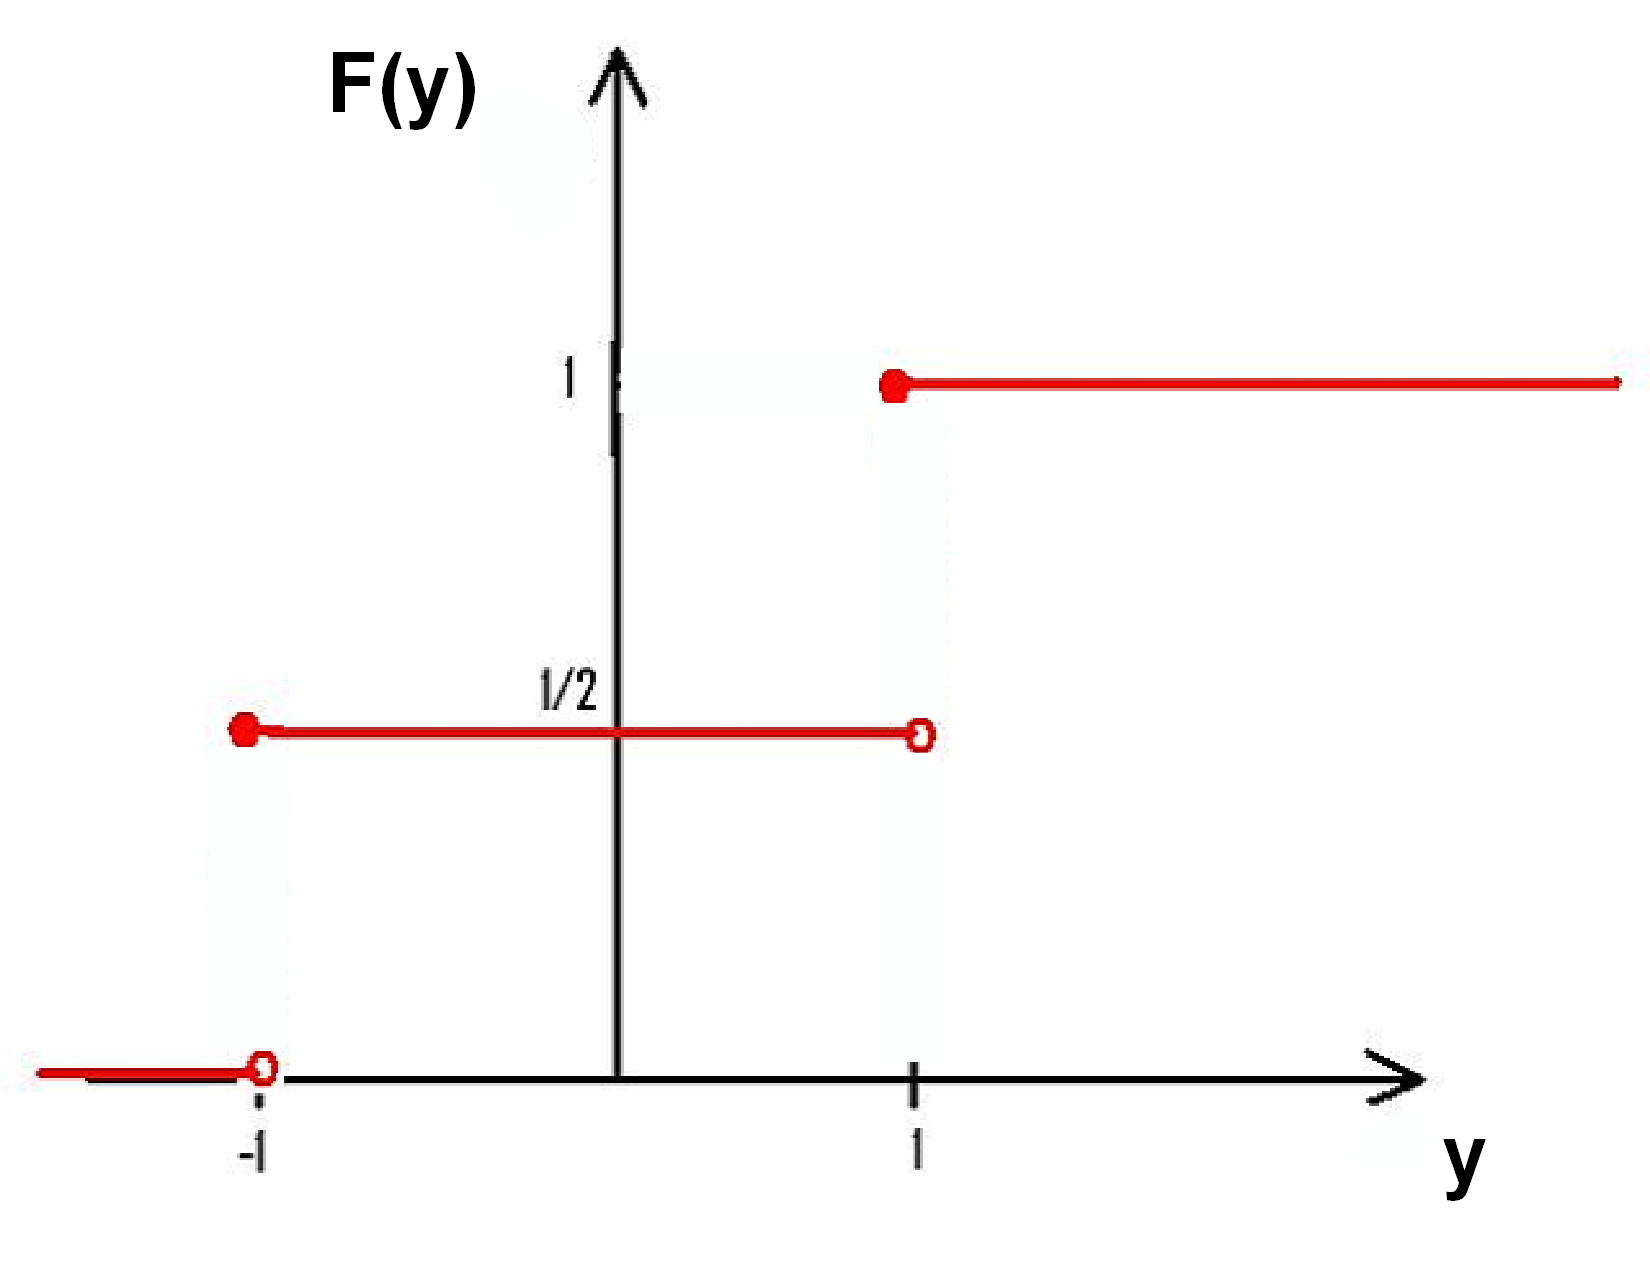
\includegraphics[height=6.8cm]{cdf-modif.pdf}}

\end{frame}

\begin{frame}[t,label=ex3]{Exemple 3}

{\small
Soit $X$ le temps de réponse (en ms) d'un serveur web à une requête. Un modèle possible pour le comportement aléatoire de $X$ est
 $$F(x)=P(X\le x)=\left\{\begin{array}{ll}
 0 & \textrm{si} \; x<0\\
 1-e^{-\lambda x} & \textrm{si} \; x\ge0,
 \end{array}\right.$$
où $\lambda$ est une constante positive, que l'on suppose connue.}

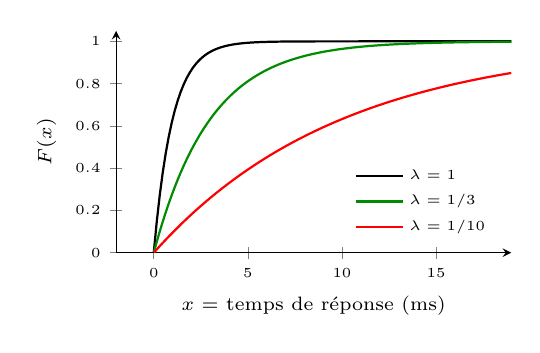
\begin{tikzpicture}
\begin{axis}[expo, ymin=0, ymax=1.05, ytick={0,0.2,0.4,0.6,0.8,1}, ylabel={$F(x)$}, legend pos=south east]
  \addplot[black, thick, domain=0:19] {1-exp(-x)}; \addlegendentry{$\lambda=1$}
  \addplot[green!55!black, thick, domain=0:19] {1-exp(-x/3)}; \addlegendentry{$\lambda=1/3$}
  \addplot[red, thick, domain=0:19] {1-exp(-x/10)}; \addlegendentry{$\lambda=1/10$}
  \addplot[black, thick, domain=-2:0, forget plot] {0};
\end{axis}
\end{tikzpicture}

\end{frame}
\begin{frame}[t]{Exemple 3 (suite)}

Supposons que $\lambda=1/10$. Calculez ces probabilités.

\begin{itemize}\itemsep=12mm
\item $P(X\leq 15)$
\item $P(X> 10)$
\item $P(5<X\leq 10)$
\end{itemize}

\vspace{5mm}
\lienreponse{rep-ex1}
\end{frame}


\begin{frame}[t,label=quizgain]{Exemple 2 : gain et fonction de répartition}

\centerline{\LARGE\bfseries\alert{QUIZ !}}
Quelle est la probabilité d'obtenir un gain supérieur à 0,75~\$?

\medskip
Répondez à l'aide de la fonction de répartition.

\vspace{5cm}
\lienreponse{rep-quiz}
\end{frame}


\begin{frame}[t]{Propriétés d'une fonction de répartition}

{\small
\begin{itemize}
 \item[1.] $0\le F_X(x)\le 1$ pour tout $x\in\mathbb{R}$
 \item[2.] $\lim\limits_{x\to\alerter{-\infty}}F_X(x)=0$ et $\lim\limits_{x\to\alerter{\infty}}F_X(x)=1$
 \item[3.] $F_X(x)$ est \alerter{non décroissante} (si $x_1\le x_2$, alors $F_X(x_1)\le F_X(x_2)$)
\end{itemize}

{\color{gray}\footnotesize Propriété plus technique : $F_X$ est aussi continue à droite,
$\lim\limits_{s\to 0^+}F_X(x+s)=F_X(x)$ pour tout $x\in\mathbb{R}$.}

\medskip

\uncover<2->{
 \begin{itemize}
  \item Pour vérifier si une fonction est une fonction de répartition, on vérifie qu'elle remplit les 3 propriétés ci-dessus.
  \item Par définition de la fonction de répartition, pour tout $a<b$, $P(a<X\le b)=F_X(b)-F_X(a)$.
 \end{itemize}
}
}
\end{frame}

\begin{frame}

\begin{Boite}{Variables aléatoires discrètes et continues}
\begin{itemize}\itemsep3mm
\item Si $F_X(x)$ est une fonction en escalier continue à droite, on dit que $X$ est une variable aléatoire \alerter{discrète}. L'ensemble de ses valeurs possibles est \alerter{dénombrable}.
\item Si $F_X(x)$ est une fonction continue, on dit que $X$ est une variable aléatoire \alerter{continue}. L'ensemble de ses valeurs possibles est \alerter{non dénombrable}.
 \end{itemize}
\end{Boite}

\end{frame}

\section{Variables aléatoires discrètes}

\begin{frame}[t]{Fonction de probabilité/masse}

 \begin{defn}{}
  Soit $X$ une v.a. \alerter{discrète}. On appelle \alerter{fonction de probabilité} (ou \alerter{fonction de masse},
  ou \alerter{fonction de masse de probabilité}; PMF, de \textit{probability mass function}) de $X$ la fonction
  $$p_X:\mathbb{R}\to[0,1]$$ qui associe la valeur
  $$p_X(x)=P(X=x)$$
  à tout $x\in \mathbb{R}$.
 \end{defn}

\end{frame}




\begin{frame}[t,label=ex2pmf]{Exemple 2 : fonctions de probabilité}

Retournons à l'exemple du dé.\\
Trouvons $p_X$ et $p_Y$.

\lienreponse{rep-ex1}
\end{frame}


\begin{frame}[t]{Exemple 2 : fonctions de probabilité (suite)}

\end{frame}



\begin{frame}[t,label=proppmf]{Propriétés de la fonction de probabilité}

Une fonction $p_X$ est une fonction de probabilité pour une v.a. discrète $X$ \alerter{si et seulement si} elle satisfait deux propriétés :

\vspace{0.2 in}

\begin{enumerate}
 \item $ $
 \vspace{0.3 in}
 \item $ $
\end{enumerate}

\lienreponse{rep-ex1}
\end{frame}

\section{Variables aléatoires continues}

\begin{frame}[t]{Fonction de densité}

\begin{defn}{}
Soit $X$ une v.a. continue. On appelle \alerter{fonction de densité} (PDF, de \textit{probability density function}) de $X$ la fonction qui associe la valeur
$$f_X(x)=\frac{d}{dx}F_X(x)$$
à tout $x\in \mathbb{R}$.
\end{defn}
\end{frame}
\begin{frame}

\begin{Boite}{Lien entre la fonction de répartition $F_X(x)$ et la fonction de densité $f_X(x)$}
Par définition de la fonction de densité $f_X(x)$, on a
\begin{align*}
 F_X(x)&=\int_{-\infty}^x f_X(u)\;du, \\
 P(a<X\le b)&=F_X(b)-F_X(a)=\int_a^bf_X(u)\;du.
\end{align*}
La probabilité qu'une variable aléatoire continue prenne une valeur dans un intervalle se calcule donc en intégrant $f_X(x)$.
\end{Boite}

\end{frame}

\begin{frame}[t]{Probabilité = aire sous la densité}

\begin{center}
\begin{tikzpicture}[xscale=0.62, yscale=0.62]
  % axes
  \draw[->] (-1.5,0) -- (10.5,0) node[below] {$x$};
  \draw[->] (0,-0.1) -- (0,3.2) node[left] {$f_X(x)$};
  % région hachurée entre a et b
  \fill[pattern=north east lines, pattern color=black!70]
    (4.6,0) -- plot[domain=4.6:6.4, samples=30] (\x,{dens(\x)}) -- (6.4,0) -- cycle;
  \draw[dashed] (4.6,0) -- (4.6,{dens(4.6)});
  \draw[dashed] (6.4,0) -- (6.4,{dens(6.4)});
  \node[below] at (4.6,0) {$a$};
  \node[below] at (6.4,0) {$b$};
  % densité
  \draw[very thick, red] (-1.5,0) -- (1,0);
  \draw[very thick, red] plot[domain=1:9, samples=80] (\x,{dens(\x)});
  \draw[very thick, red] (9,0) -- (10.3,0);
  % image de X
  \draw[<->] (1,-0.9) -- (9,-0.9) node[midway, below] {$\mathbb{R}_X$};
  \draw (1,-0.75) -- (1,-1.05); \draw (9,-0.75) -- (9,-1.05);
\end{tikzpicture}
\end{center}

$f_X(x)$ n'est \alerter{pas} une probabilité, mais son intégrale sur un intervalle donne la
probabilité que $X$ prenne une valeur dans cet intervalle.

Autrement dit, $f_X(x) \alerter{\neq} P(X=x)$.

\end{frame}

\begin{frame}[t]{Propriétés d'une fonction de densité}

\begin{itemize}
 \item[1.] $f_X(x)\ge0$ pour tout $x\in\mathbb{R}$
 \item[2.] $\displaystyle\int_{-\infty}^\infty f_X(x)\;dx=1$
 \item[3.] $f_X(x)$ est continue par morceaux
 \item[4.] si $x\notin \mathbb{R}_X$, alors $f_X(x)=0$
\end{itemize}

{\color{gray}\small Attention : $f_X(x)$ n'est pas une probabilité; elle peut être supérieure à 1.}

\uncover<2->{
Comme $\displaystyle\int_a^af_X(u)\;du=0$,
on a $P(X=a)=0$ pour tout $a\in\mathbb{R}$ dans le cas
d'une v.a. \underline{continue}. Par conséquent,
$$
\left.\begin{array}{l}
P(a<X<b)\\P(a<X\le b)\\P(a\le X<b)\\P(a\le X\le b)
\end{array}\right\}=\int_a^bf_X(u)\;du.$$}

\end{frame}

\begin{frame}[t,label=ex4]{Exemple 4}

\centerline{\LARGE\bfseries\alert{QUIZ !}}

{\small
Soit $X$ une v.a. continue qui peut prendre n'importe quelle valeur dans l'intervalle
$[0,20]$. On vous dit que
\begin{itemize}
\item tous les intervalles de même longueur dans $[0,10)$ sont équiprobables,
\item tous les intervalles de même longueur dans $[10,20]$ sont équiprobables,
\item un intervalle de $[10,20]$ est deux fois plus probable qu'un intervalle de même longueur dans $[0,10)$.
    \end{itemize}
\medskip
a) Déterminez la densité de $X$.}
\lienreponse{rep-quiz}
\end{frame}

\begin{frame}[t]{Exemple 4 (suite)}
b) Déterminez la fonction de répartition de $X$.
\lienreponse{rep-quiz}
\end{frame}

\begin{frame}[t]{Exemple 4 (suite)}
c) Évaluez $P(5<X<12)$.
\lienreponse{rep-quiz}
\end{frame}


\begin{frame}[t,label=ex5]{Exemple 5 : retour au temps de réponse}
La fonction de répartition du temps de réponse $X$ (en ms) du serveur
est $F(x)=1-e^{-\lambda x}$ si
$x\ge0$, et $0$ ailleurs.
\begin{itemize}\itemsep 2cm
\item Quelle est la densité de $X$?
\item Quelle est la probabilité que le temps de réponse dépasse 5~ms?
\end{itemize}
\lienreponse{rep-ex2}
\end{frame}

\begin{frame}[t,label=quizmemoire]{Exemple 5 (suite)}

\centerline{\LARGE\bfseries\alert{QUIZ !}}
\begin{itemize}
\item Une requête attend sa réponse depuis 5~ms. Quelle est la probabilité que la réponse arrive entre 10 et 15~ms?
\end{itemize}
\lienreponse{rep-quiz}
\end{frame}


\begin{frame}[t,label=quizassoc]{Densités et fonctions de répartition}

\centerline{\LARGE\bfseries\alert{QUIZ !}}
Associez chaque densité à la bonne fonction de répartition.
\begin{center}
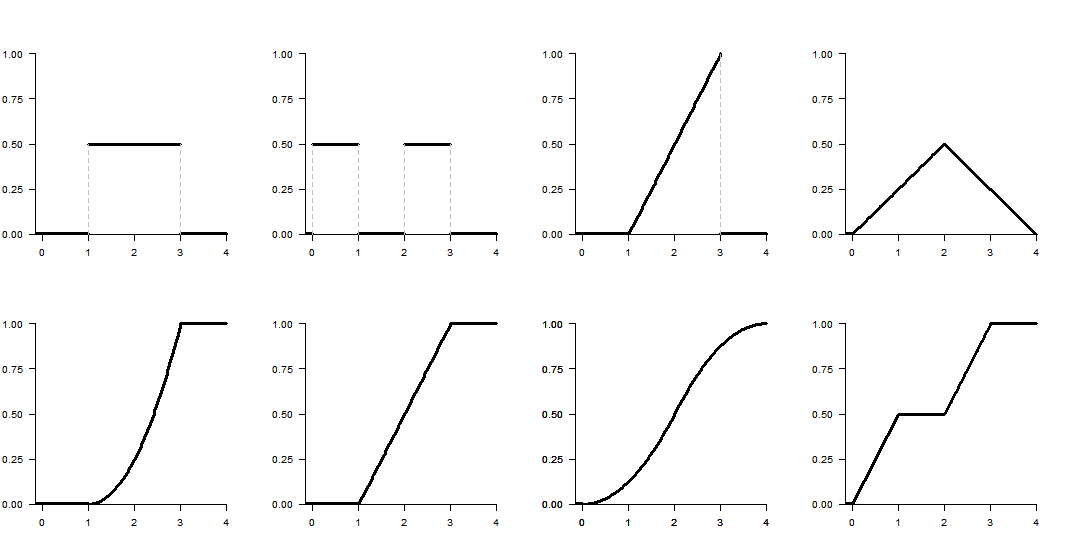
\includegraphics[width=11.4cm]{association.png}
\end{center}
\lienreponse{rep-quiz}
\end{frame}

\section{Espérance et variance d'une variable aléatoire}

\begin{frame}[t]{Aspects importants d'une distribution}
Les fonctions de répartition, de densité et de probabilité décrivent complètement la distribution d'une variable aléatoire. Il est tout de même utile de résumer les principaux aspects de son comportement :

\medskip
\begin{itemize}\itemsep2mm
\item la tendance centrale;
\item la dispersion;
\item la forme.
\end{itemize}

À partir de maintenant, quand une seule variable aléatoire est à l'étude, nous écrirons $F(x)$, $p(x)$ et $f(x)$ au lieu de $F_X(x)$, $p_X(x)$ et $f_X(x)$.

\end{frame}

\begin{frame}[t]{Mesure de la tendance centrale}
\begin{defn}{}
 L'\alerter{espérance} (moyenne théorique) d'une variable aléatoire $X$ est donnée par
 $$E(X)=\sum_{x\in \mathbb{R}_X} x\, p(x)$$
 pour une variable aléatoire discrète,

 ou
 $$E(X)=\int_{-\infty}^\infty x f(x)\;dx$$
 pour une variable aléatoire continue.
\end{defn}
La notation la plus fréquente est $E(X)=\mu$.
\end{frame}

\begin{frame}[t,label=exde]{Exemple : espérance du résultat d'un dé}
On lance un dé équilibré à 6 faces. Soit $X$ le résultat obtenu.

\medskip
Calculez $E(X)$.
\lienreponse{rep-ex2}
\end{frame}

\begin{frame}[t]{Interprétation de l'espérance de $X$}
    C'est la valeur moyenne que l'on obtiendrait si on répétait l'expérience aléatoire une infinité de fois.

\vspace{1cm}

    Pour une variable aléatoire continue, la moyenne d'un nombre fini de répétitions ne sera en pratique jamais exactement égale à l'espérance.

\vspace{1cm}

    Pour une variable aléatoire discrète, ce n'est pas toujours le cas. Un exemple?
\end{frame}

\begin{frame}[t,label=ex6]{Exemple 6 : retour au temps de réponse}
\begin{columns}[T]
\begin{column}{0.42\textwidth}
{\small
$f(x)=\left\{\begin{array}{cl}\lambda e^{-\lambda x}&\text{si} \;x>0\\
 0&\text{si} \; x\leq 0
 \end{array}\right.$

\vspace{3mm}

Quel est le temps de réponse moyen du serveur? (Répondez pour $\lambda$ en général, sans fixer de valeur.)
}
\end{column}
\begin{column}{0.55\textwidth}
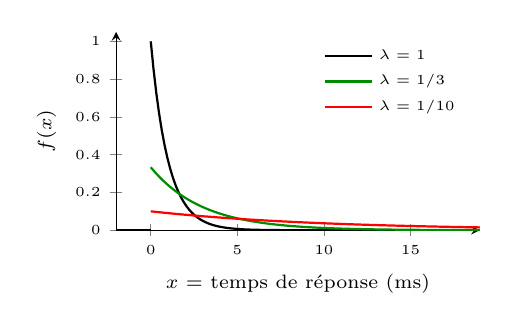
\begin{tikzpicture}
\begin{axis}[expo, width=6.2cm, height=4.1cm, ymin=0, ymax=1.05, ytick={0,0.2,0.4,0.6,0.8,1}, ylabel={$f(x)$}, legend pos=north east]
  \addplot[black, thick, domain=0:19] {exp(-x)}; \addlegendentry{$\lambda=1$}
  \addplot[green!55!black, thick, domain=0:19] {exp(-x/3)/3}; \addlegendentry{$\lambda=1/3$}
  \addplot[red, thick, domain=0:19] {exp(-x/10)/10}; \addlegendentry{$\lambda=1/10$}
  \addplot[black, thick, domain=-2:0, forget plot] {0};
\end{axis}
\end{tikzpicture}
\end{column}
\end{columns}
\lienreponse{rep-ex2}
\end{frame}

\begin{frame}[t]{Variabilité d'une variable aléatoire}

Deux variables aléatoires peuvent avoir la \underline{même espérance}
 tout en étant l'une \underline{beaucoup plus variable
 que l'autre}, c'est-à-dire avoir tendance à prendre des valeurs
 plus éloignées de son espérance.

 \medskip
 {\bf \underline{Expérience}} : on lance 30 dés équilibrés.

 $X_1=$ la valeur indiquée par le premier dé\\
 $X_2=$ la moyenne des 30 dés (leur somme divisée par 30)

 \medskip
 On peut montrer que $X_1$ et $X_2$ ont la même
 espérance (3,5).

 \medskip
 Cependant, $X_2$ aura tendance à prendre
 des valeurs très proches de 3,5, alors que $X_1$ prend
 n'importe quelle valeur entre 1 et 6 avec la même probabilité.

\end{frame}

\begin{frame}[fragile]
\frametitle{Petite simulation}
{\small
Voici 12 répétitions de cette expérience, simulées avec \texttt{R} :

\begin{verbatim}
      X1            X2
 [1,]  2       3.633333
 [2,]  6       3.666667
 [3,]  4       3.933333
 [4,]  4       3.633333
 [5,]  5       3.833333
 [6,]  6       3.600000
 [7,]  6       3.400000
 [8,]  3       3.166667
 [9,]  2       3.766667
[10,]  5       3.066667
[11,]  3       3.566667
[12,]  1       3.300000
\end{verbatim}
}
\end{frame}

\begin{frame}[t]{Fonctions de probabilité de $X_1$ et $X_2$}

{\small La figure ci-dessous montre la fonction de probabilité de $X_1$
en bleu et celle de $X_2$ en rouge. Même si les deux v.a. ont la même
espérance, la distribution de $X_2$ est beaucoup
plus concentrée autour de 3,5 que celle de $X_1$.

\centerline{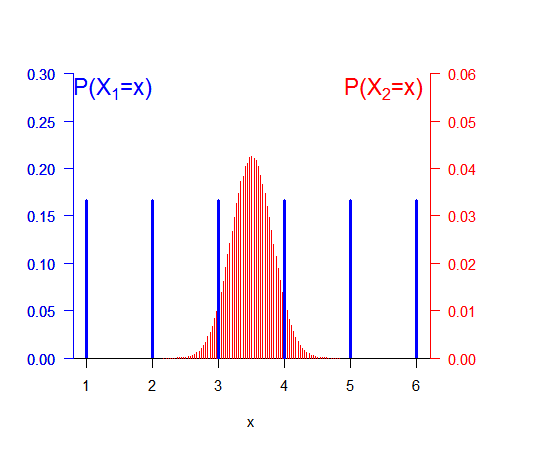
\includegraphics[height=2.1in]{pmf-x1x2-modif.png}}
}
\end{frame}

\begin{frame}[t]{Mesure de dispersion d'une distribution}

\begin{defn}{}
La \alerter{variance} d'une variable aléatoire $X$ est donnée par
  $$V(X)=\sum_{x\in \mathbb{R}_X} (x-\mu)^2p(x)$$
pour une variable aléatoire discrète, et
  $$V(X)=\int_{-\infty}^\infty (x-\mu)^2f(x)\;dx$$
pour une variable aléatoire continue.
\end{defn}
La notation la plus fréquente est $V(X)= \sigma^2$.
On en tire l'\alerter{écart-type}, $\sigma = \sqrt{V(X)}=\sqrt{\sigma^2}$.

\end{frame}


\begin{frame}[t,label=ex7]{Exemple 7 : retour au temps de réponse}

Le temps de réponse de ce serveur est-il très variable?
\lienreponse{rep-ex2}
\end{frame}

\section{Espérance d'une fonction d'une variable aléatoire}

\begin{frame}[t]{Espérance d'une fonction d'une variable aléatoire}

{\small
\begin{Boite}{Espérance d'une fonction d'une variable aléatoire}
 Soit $X$ une v.a. et posons $Y=H(X)$, une fonction
 de $X$. L'\alerter{espérance
 de $H(X)$} (ou de $Y$) est définie par
 $$E(Y)=E\bigl(H(X)\bigr)=\sum_{x\in\mathbb{R}_X}H(x)\,p(x)$$
 ou
 $$E(Y)=E\bigl(H(X)\bigr)=\int_{-\infty}^\infty H(x)f(x)\;dx.$$
\end{Boite}
Un cas particulier :
\begin{itemize}
 \item $H(X)=(X-\mu)^2\Rightarrow E\bigl((X-\mu)^2\bigr)=V(X)=\sigma^2$, la variance de $X$.
\end{itemize}
}
\end{frame}

\begin{frame}[t]{Résultats utiles}

Supposons que $a$ et $b$ sont des constantes.

\begin{itemize}
\item<1-> $E(aX+b)=aE(X)+b$\ \ \ \ \

\vspace{0.45in}

\item<1-> $V(X)=E(X^2)-\bigl(E(X)\bigr)^2$\ \ \ \ \

\vspace{0.75in}

\item<1-> $V(aX+b)=a^2V(X)$\ \ \ \ \
\end{itemize}
\end{frame}

\begin{frame}[t,label=preuve1]
Prouvez que $E(aX+b)=aE(X)+b$ dans le cas d'une variable aléatoire continue.
\lienreponse{rep-ex2}
\end{frame}

\begin{frame}[t]
Prouvez que $V(X)=E(X^2)-\bigl(E(X)\bigr)^2$.
\lienreponse{rep-ex2}
\end{frame}

\begin{frame}[t]
Prouvez que $V(aX+b)=a^2V(X)$.
\lienreponse{rep-ex2}
\end{frame}

\begin{frame}[t,label=ex8]{Exemple 8 : retour au temps de réponse}

Un service infonuagique facture chaque requête 10~¢, plus 3~¢ par milliseconde de temps de réponse.
Le coût d'une requête (en ¢) est donc $C=10+3X$, où $X$ est le temps de réponse.
Quels sont le coût moyen et l'écart-type du coût d'une requête?

Rappel : $E(X)=1/\lambda\qquad V(X)=1/\lambda^2$
\lienreponse{rep-ex2}
\end{frame}



\section{Réponses des exemples}

\begin{frame}[t,label=rep-ex1]{Réponses des exemples (1/2)}
\footnotesize
\begin{itemize}
\item \retour{ex2tab}{Exemple 2 (suite)} (tableau de $X(e)$ et $Y(e)$) : $X(e)=e$ pour $e=1,\ldots,6$~;
$Y(e)=-1$ si $e\in\{1,2,3\}$, $Y(e)=1$ si $e\in\{4,5,6\}$.
\item \retour{ex2prob}{Exemple 2 : probabilités} (perdre 1~\$) : $P(Y=-1)=P(e\in\{1,2,3\})=3/6=1/2$.
\item \retour{ex2rep}{Exemple 2 : fonction de répartition} de $Y$ : $F_Y(y)=0$ si $y<-1$~;
$F_Y(y)=1/2$ si $-1\le y<1$~; $F_Y(y)=1$ si $y\ge1$.
\item \retour{ex3}{Exemple 3 (suite)} ($\lambda=1/10$) : $P(X\le15)=1-e^{-1{,}5}\approx0{,}777$~;
$P(X>10)=e^{-1}\approx0{,}368$~; $P(5<X\le10)=e^{-0{,}5}-e^{-1}\approx0{,}239$.
\item \retour{ex2pmf}{Exemple 2 : fonctions de probabilité} : $p_X(1)=\cdots=p_X(6)=1/6$~; $p_Y(-1)=p_Y(1)=1/2$.
\item \retour{proppmf}{Propriétés de la fonction de probabilité} : (1) $p_X(x)\ge 0$ pour tout $x$~; (2) $\sum_x p_X(x)=1$.
\end{itemize}

\end{frame}

\begin{frame}[t,label=rep-ex2]{Réponses des exemples (2/2)}
\footnotesize
\begin{itemize}
\item \retour{ex5}{Exemple 5} (retour au temps de réponse) : $f(x)=\lambda e^{-\lambda x}$ si $x>0$ (0 sinon)~;
$P(X>5)=e^{-5\lambda}$.
\item \retour{exde}{Exemple} (espérance d'un dé) : $E(X)=(1+2+\cdots+6)/6=3{,}5$.
\item \retour{ex6}{Exemple 6} : $E(X)=1/\lambda$.
\item \retour{ex7}{Exemple 7} : $V(X)=1/\lambda^2$~; plus $\lambda$ est petit, plus $X$ est variable.
\item \retour{preuve1}{Preuves} (\enquote{Résultats utiles}) : découlent directement des définitions de $E(\cdot)$ et $V(\cdot)$ en substituant $aX+b$, puis, pour la deuxième, en développant $(X-\mu)^2=X^2-2\mu X+\mu^2$.
\item \retour{ex8}{Exemple 8} : $E(C)=10+3/\lambda$, $V(C)=9/\lambda^2$, donc l'écart-type est $3/\lambda$.
\end{itemize}

\end{frame}

\section{Réponses des quiz}

\begin{frame}[t,label=rep-quiz]{Réponses des quiz}
\footnotesize
\begin{itemize}
\item \retour{quizgain}{Quiz} (dé, gain $>0{,}75$~\$) : $P(Y>0{,}75)=1-F_Y(0{,}75)=1-1/2=1/2$.
\item \retour{ex4}{Quiz} (Exemple 4, densité sur $[0,20]$) : $f(x)=1/30$ si $x\in[0,10)$, $f(x)=1/15$ si
$x\in[10,20]$, 0 sinon~; $F(x)=x/30$ si $0\le x<10$, $F(x)=1/3+(x-10)/15$ si $10\le x\le20$~;
$P(5<X<12)=3/10=0{,}3$.
\item \retour{quizmemoire}{Quiz} (temps de réponse, $P(10<X<15\mid X\ge5)$) : par la propriété d'absence de mémoire,
$=e^{-5\lambda}-e^{-10\lambda}$.
\item \retour{quizassoc}{Quiz} (association densité-répartition) : densité 1 (uniforme sur $[1,3]$)
$\leftrightarrow$ répartition 2 (rampe linéaire)~; densité 2 (deux blocs sur $[0,1]$ et $[2,3]$)
$\leftrightarrow$ répartition 4~; densité 3 (rampe croissante sur $[1,3]$) $\leftrightarrow$ répartition 1
(courbe convexe)~; densité 4 (triangulaire sur $[0,4]$) $\leftrightarrow$ répartition 3 (courbe en S).
\end{itemize}

\end{frame}

\begin{frame}{Bibliographie}
 	Ce document est rédigé avec Beamer ainsi qu'une classe .cls fournie par Jérôme Soucy. Les diapositives sont adaptées des diapositives créées par Anne-Sophie Charest
 pour le cours STT-1000 ainsi que celles créées par Thierry Duchesne et Emmanuelle Reny-Nolin pour le cours STT-1900.
 	\printbibliography
 	\vfill
 	\footnotesize Pour signaler une erreur dans ce document, veuillez écrire à l'adresse :~\href{mailto:julien.miron@mat.ulaval.ca}{julien.miron@mat.ulaval.ca}.
 \end{frame}

\end{document}
